\documentclass[10pt,a4paper]{article}
\usepackage[utf8]{inputenc}
\usepackage{amsmath}
\usepackage{amsfonts}
\usepackage{amssymb}
\usepackage{graphicx}
\usepackage{fullpage}

\newenvironment{boxed2}
    {\begin{center}
    \begin{tabular}{|p{\textwidth}|}
    \hline \\
    }
    { 
    \\ \\ \hline
    \end{tabular} 
    \end{center}
    }


\begin{document}
\section{Introduction}
Traditional  machine learning methods applied to the material sciences have often predicted invariant, scalar properties of material systems to great effect. Newer, coordinate equivariant models promise to provide a coordinate system dependent output in a well defined manner, but recent applications often neglect a direct prediction of directional (i.e. coordinate system dependent) quantities and instead are used to predict still just invariant quantities.

In such rotationally equivariant models, features are often associated with irreducible representations of the rotation group. This association may be leveraged to predict tensorial quantities directly from the outputs of such models.
This component-wise prediction of tensorial properties is achieved by decomposing tensors into harmonic subspaces via a \textit{tensor spherical harmonic decomposition}, by which we may also associate arbitrary tensors with the irreducible representations of the rotation group. This essentially allows us to read off tensors component-wise from the representations learned from equivariant models.

In this work, we present results for the prediction of various tensors describing material properties directly from crystalline structures using such rotationally equivariant models. Namely, given some material's crystalline structure, we may predict tensor components of dielectric, piezoelectric, and elasticity tensors directly from the output of a $SE(3)$ equivariant model.

Below, we give explicit decompositions of the relevant tensors and a brief overview of the tools used. We then present results for some basic implementations of such an approach, and attempt some transfer learning applications

\section{$SO(3)$ Equivariant Neural Networks}
Neural networks are a class of universal function approximators, composed layer-wise by functions $\mathcal{L}^1\circ\mathcal{L}^2\circ ... \circ \mathcal{L}^n $, where each layer-to-layer transition map $\mathcal{L}^i$ is a trainable function from some feature space associated with layer $L$ to a feature space associated with layer $L+1$.

Many modern approaches use a specific type of neural network, referred to as a Graph Neural Network (GNN), which act on data encoded in features associated with some representative graph (i.e. a collection of nodes and connections between them), while preserving the underlying connectivity of the graph representation.

Basic graph networks however are, in general, rotationally invariant. As such, these models are incapable of predicting any coordinate-system quantities, such as tensor components. 
\begin{center}
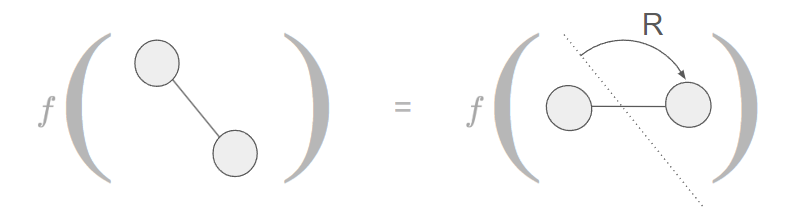
\includegraphics[scale=0.8]{invariant.png}
\end{center}
In an $SO(3)$-network, however, features are further associated with $SO(3)$ irreducible representation: namely, spherical harmonics $Y_{\ell}^m$, which are doubly indexed the rotational order $\ell\geq 0$, and the azimuthal order $-\ell\leq m \leq \ell$.

Thus, a traditional feature set $V^{(n)a}$ of channel $a$ and associated with object $n$, has an additional two indices $\ell$ and $m$ in an $SO(3)$ network, corresponding to the aformentioned indices of a harmonic expansion.

\begin{figure}
\begin{center}
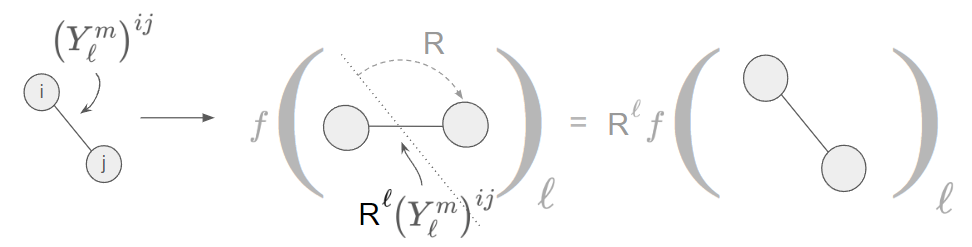
\includegraphics[scale=0.8]{equivariant.png}
\end{center}
\caption{Example diagram showcasing a rotationally equivariant update scheme where features are associated with spherical harmonics (indexed by $\ell$ and $m$). Note that the function $f$'s output also has a corresponding $\ell$ index, as well as the rotation operator $R^{\ell}$.}
\end{figure}

\subsection{Equivariant Layers}
Compositions of equivariant functions are themselves equivariant functions. As such, we may form an equivariant network by composing it layer-wise from a set of common equivariant functions.

Here, we consider three types of $SO(3)$-equivariant functions from which we may compose our equivariant networks: namely, $SO(3)$-feature convolutions, $\ell$-wise self-interactions and non-linearities, and pooling. An overview of each is given below.

\subsubsection{$SO(3)$ Convolution}
Note here that the tensor product of two representation spaces is equivariant under transformation of the two subspaces, i.e.:
$$
\mathcal{D}^V\otimes \mathcal{D}^W=\mathcal{D}^{V\otimes W}
$$
Tensors products of $SO(3)$ representations are cleanly related to a third set of $SO(3)$ representations by way of Clebsch-Gordan coefficients $c^{\ell_3m_3}_{\ell_1m_1\ell_2m_2}$ as:
$$
(u\otimes v)_{\ell_o}^{m_o} = c_{\ell_1m_1\ell_2m_2}^{\ell_om_o}u_{\ell_1}^{m_1}v_{\ell_2}^{m_2}
$$
where $u$ and $v$ are harmonic vectors of order $\ell_1$ and $\ell_2$, respectively.

Thus, we maintain equivariance by defining convolution to be the scaled tensor product of the two representation spaces (i.e. that of the input feature space, and the filter space), so that layer to layer convolutional maps $\mathcal{L}$ may be defined component-wise as:
$$
\mathcal{L}^{\ell_o}_{acm_o}\big(\vec{r}_a,V_{acm_i}^{\ell_i}\big) = \sum_{m_f,m_i}c_{\ell_im_i\ell_fm_f}^{\ell_o m_o}\sum_{b}F^{\ell_f\ell_i}_{cm_f}(r_{ab})V_{bcm_i}^{\ell_i}
$$
where the filter function $F^{\ell_f\ell_i}_{cm_f}(r_{ab})$ depends only on the distance between point $a$ and $b$ (as opposed to directional dependence, to maintain equivariance), but has independent, trainable parameters for different rotational orders $\ell_f, \ell_i$, azimuthal orders $m$, and channels $c$.

To maintain equivariance, for an input feature set of the type described above,  through convolution with some filter $F$,  the filter also must be associated with a set of spherical harmonics, and thus also has an additional two indices $\ell_f$ and $m_f$. 


\subsubsection{Self-Interaction}
Feature sets for individual objects may also update according to themselves as long as they act across $m$ for every $\ell$ and only update according to the different channels $c$. That is, functions of the form:
$$
V_{acm}^{\ell} \rightarrow  \sum _{c}W^{\ell}_{c'c}V_{acm}^{\ell}
$$
are also equivariant. 

\subsubsection{Non-Linearities}
We can also apply point-wise non linearities and maintain equivariance, as long as they also respect the across $m$ indices for every order feature $\ell$.

\subsubsection{Pooling}
Pooling, or aggregation, across all elements or objects (index $a$) while preserving the $m$ and $\ell$ indices is itself equivariant. Thus, functions of the form:
$$
 M_{cm}^{\ell} = \text{AGG}_{a}(\lbrace V_{acm}^{\ell}\rbrace)
$$ 
where $\text{AGG}$ is an arbitrary aggregation function performed only over the object index $a$, are also available in the construction of $SO(3)$ networks.
 
\subsubsection*{SO(3) Equivariant Outputs}
The outputs of these networks are also associated with some indices $\ell$ and $m$ of course, and thus are also associated with some set of spherical harmonics.

Such $SO(3)$ equivariant networks are then naturally well suited for the prediction of tensorial properties. Since tensors may generally be decomposed into a set of $SO(3)$ invariant subspaces which can then each be associated with a set of spherical harmonic tensors. Since the outputs of $SO(3)$ networks naturally transform like spherical harmonic tensor coefficients indexed by $\ell$ and $m$, we may then essentially read them off as such and convert back into Cartesian form.

\section{Spherical Harmonic Tensors and $SO(3)$ Invariant Subspaces}\label{so3inv}
We may construct a set of spherical harmonic tensors $\hat{Y}_{\ell}^m$ by first defining the $J_z$ vector basis and then considering symmetric products of such vectors. We define the $J_z$ basis:
$$
\begin{bmatrix}
a_+ \\
a_0 \\
a_-
\end{bmatrix}=\begin{bmatrix}
-\frac{1}{\sqrt{2}} & -\frac{i}{\sqrt{2}} & 0\\
 0 & 0 & 1\\
-\frac{1}{\sqrt{2}} & +\frac{i}{\sqrt{2}} & 0\\
\end{bmatrix}\begin{bmatrix}
x \\
y \\
z
\end{bmatrix}
$$
where $x,y,z$ are Cartesian components of the same vector. In this basis, the unit vectors associated with these components correspond to unit vector spherical harmonics $\hat{Y}_{\ell=1}^m$ (where we will assume Racah normalization for all definitions).

Now, recall the Clebsch-Gordon expansion of products of spherical harmonics (again, in the Racah normalization):
$$
Y_{\ell_1}^{m_1}\otimes Y_{\ell_2}^{m_2} = \sum_{L=-|\ell_1-\ell_2|}^{\ell_1+\ell_2}\sum_{M=-L}^{L}c_{\ell_1 0 \ell_2 0}^{L0}c_{\ell_1 m_1 \ell_2 m_2}^{LM}Y_{L}^M.
$$
This may be used to draw a correspondence between symmetrized tensor products of $n$ vectors in the $J_z$ and rank $\leq n$ spherical harmonic tensors. The coefficients for such a transformation relevant for the tensors considered here are listed in \textbf{Appendix \ref{cgcoef}}

The spherical harmonics $Y_{\ell}^m$ canonically refer to a complex basis, as should be clear from our definition of the $J_z$ basis. Many tensors describing macroscopic responses of materials are strictly real-valued however. Hence, we may desire to then transform into a set of real-valued spherical harmonics.

Thus, we may decompose an arbitrary tensor of rank-$n$ into a set of symmetric tensors of rank-$\ell$ with $0\leq\ell\leq n$, and then use the relations between the $J_z$ basis components and the spherical harmonic components $y_{\ell}^m$. We then may arrive at a set of real spherical harmonic components $y_{\ell m}$ using the relations specified in \textbf{Appendix \ref{realsph}}.


However, since this correspondence can only be drawn for symmetric tensors, for any arbitrary tensor we first need some way to describe it in terms of a set of symmetric tensors. The above approach can then be applied to this set of symmetric components.

This decomposition of an arbitrary rank tensor into a set of invariant symmetric subspaces is equivalent to an $SO(3)$ decomposition of a tensor space. Such $SO(3)$ invariant subspaces can be constructed via a compound decomposition with respect to $GL$, $SL$, and $O$: which result from application of Young symmetrizers, contractions with the totally antisymmetric $\epsilon$, and contractions with the totally symmetric $g$, respectively.

For example, for a rank-two tensor, we may always decompose it with respect to GL first (by using the corresponding Young symmetrizers), resulting in a symmetric tensor $S$ and antisymmetric tensor $A$.
\begin{center}

\medskip

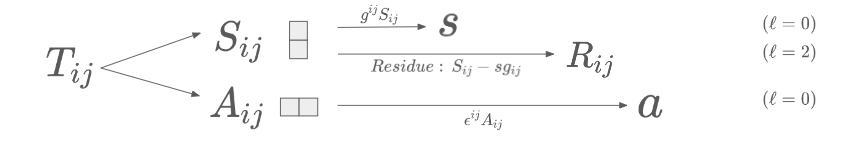
\includegraphics[scale=1.1]{rank2.png}
\end{center}
The symmetric $S$ then has an invariant rank-0 space, commonly referred to as it's trace, and constructed via total contraction with the metric tensor $g_{ij}$. The traceless residue of $S$ then is a symmetric, rank-2 tensor which is itself an invariant subspace. The antisymmetric $A$ then may be fully contracted with the totally antisymmetric $\epsilon_{ij}$ to return another rank-0 invariant subspace.

The relevance of these facts is that, in the manner described above, we are able to decompose an arbitrary tensor into a set of components that transform like spherical harmonics, just like the representations in $SO(3)$ equivariant models. We now give spherical harmonic decompositions of several tensors describing common material properties, and then use these decompositions to predict these tensors directly from material structure.


\section{Spherical Harmonic Decomposition of Common Material Property Tensors}

We now give a brief overview of the harmonic decomposition of three common material properties described by tensors: the dielectric tensor $\epsilon$, the piezoelectric strain tensor $d$, and the elasticity tensor $C$. A full overview of each decomposition is given in Appendix \ref{decomps}.

\subsection{Dielectric Tensors}
The dielectric permittivity tensor  $\mathbf{\epsilon}$ of some material is a linear model of it's electric displacement $\vec{D}$ in response to an external electric field $\vec{E}$:
$$
\vec{D}=\mathbf{\epsilon}\vec{E}
$$
Note that here we focus only on static responses, that is, $(\partial/\partial t)\vec{E}=0$, due to the restriction of data to this case. 

The dielectric tensor $\epsilon$ then is a rank-two tensor formed from vector spaces over the field $\mathbb{R}^3$, where we henceforth ignore the distinction between co- and contravariant components due to the Euclidean structure $g_{ij}=\delta_{ij}$.

The dielectric tensor  $\epsilon$ is symmetric under permutation of it's indices, such that:
$$
\epsilon_{ij}=\epsilon_{ji}.
$$
The dielectric tensor then may be decomposed further into it's trace $g_ij\epsilon_ij$ and it's traceless residue $R_{ij}$, resulting in two invariant subspaces of rank-0 and 2, respectively. These two symmetric subspaces then admit a decomposition in the manner described in Section \ref{so3inv}.

\subsection{Piezoelectric Tensors}
The piezoelectric strain constants $(d_{ijk})_{T}$ are defined (at constant temperature) by the thermodynamic relation:
$$
\big(d_{ijk}\big)_{T}=\left(\frac{\partial \epsilon_{ij}}{\partial E_k} \right)_{\sigma, T}
$$
where $\epsilon$ is the strain tensor, and the partial derivative is taken at constant stress $\sigma$ and temperature $T$.

These strain constants $d_{ijk}$ are related to the piezoelectric stress constants $e_{ijk}$ via the elastic tensor $C_{ijkl}$ according to:
$$
\big(e_{ijk}\big)_T=\big(d_{ilm}\big)\big(C_{ijkl}\big)_{E,T}
$$
\begin{center}
with $e_{ijk}$ defined as:
\end{center}
$$
\big(e_{ijk}\big)_{T}=\left(\frac{\partial D_{i}}{\partial \epsilon_{jk}} \right)_{\sigma, T}
$$
and where $D$ is the resulting electric displacement vector in the material. We now will generally neglect the explicit notation of constant parameters.

The piezoelectric strain components $d_{ijk}$ are symmetric under $i,j$ due to the symmetry of the strain tensor $\epsilon_{ij}$, so that we have:
$$
d_{ijk}=d_{jik}.
$$
This symmetry gives us a natural $GL$ decomposition into the totally symmetric $S$ and the mixed-symmetry $A$, defined component-wise from $d$ as:

\begin{align*}
S_{ijk}&=\frac{1}{3}\big(d_{ijk}+d_{ikj}+d_{kji}\big)\\
A_{ijk}&=\frac{1}{3}\big(2d_{ijk}-d_{ikj}-d_{kji}\big).\\
\end{align*}

The fully symmetric part $S$ then consists of a trace vector$g_{ij}S_{ijk}$, and a symmetric residue $W$; which correspond to the spaces  $\mathcal{H}^{(1)}$ and $ \mathcal{H}^{(3)}$, respectively.

The mixed symmetry part $A$ requires decomposition with respect to $SO(3)$, so that we have a set of symmetric tensors describing it. It's 8 independent components can be described by a $5\oplus 3$ dimensional space consisting of a symmetric rank-2 tensor and a trace vector.

The trace vector $v^i$, describing $A$'s 3-dimensional $SO(3)$ invariant subspace, can be formed from the contraction of the metric tensor $g$ along $A$'s first and second indices. That is, we define:
$$
v^i =g_{jk}A^{ijk}
$$
Note that this choice is somewhat arbitrary, since we could define the trace part to correspond to the contraction along the first and third indices, or the second and third. However, it can be shown that for the mixed symmetry of $A$, these two potential trace vectors are linearly dependent (related by an overall factor of $1$ and $-2$, respectively).

Rather simply then, we can reconstruct a third-rank tensor $V$, corresponding to this rank-one invariant subspace, by defining $V$ component-wise as:
$$
V_{ijk} =\frac{1}{4}\big[v_i g_{jk}+ v_j g_{ik} - 2 v_j g_{ik}\big]
$$
The rank-2 invariant subspace of $A$ then may be constructed by symmetrizing the partial contraction with $\epsilon$ along the first and second indices (the anti-symmetric pair). Note that the antisymmetric part of this partial contraction corresponds to the trace vector space accounted for here by $u$. Explicitly, we define:
$$
b_{ij}=\frac{1}{2}\big(\epsilon_{i}^{mk}A_{mkj}+\epsilon_{j}^{mk}A_{mki}\big)
$$
which is a traceless symmetric rank-2 tensor. And from which we may reconstruct the corresponding rank-3 tensor $B$, defined by:
$$
B_{ijk}=\frac{1}{3}\big[ \epsilon_{ik}^p b_{pj}+\epsilon_{ij}^p b_{pk}\big]
$$
Thus, we may provide a total harmonic decomposition for $A$ in terms of the invariant subspaces of the rank-1 $u$ and the rank-2 $b$, such that:
$$
A_{ijk} = V_{ijk} + B_{ijk}
$$
And so, as mentioned above, the symmetric part $S$ is readily decomposed in the spherical bases into $\mathcal{H}^{(1)}\oplus \mathcal{H}^{(3)}$. And then the mixed-symmetry part inhabits the space $\mathcal{H}^{(1)}\oplus \mathcal{H}^{(2)}$.




\subsection{Elasticity Tensor}
 
 

The elasticity (or simply, elastic) tensor $C$ of a material relates it's Cauchy strain  to some small applied stress . This may be described, component-wise, as the linear relation below:
$$
\epsilon_{ij}=C_{ijkl}\tau_{kl}
$$
As should be clear by the number of indices, the elastic tensor is a fourth rank tensor. The symmetries of the elastic tensor are discussed below, as they are relevant for our application. However, it is worth noting here that the total number of independent components of the elastic tensor is 21 in general.

The elastic tensor has several symmetries, but is not, in general, symmetric upon any swapping of indices. For all systems, $C$ satisfies the so-called 'minor symmetries' below:
$$
C_{ijkl}=C_{jikl}
$$

$$
C_{ijkl}=C_{ijlk}
$$
resulting from the symmetry of the strain and stress tensors ($\tau_{ij}=\tau_{ji}$ and $\epsilon_{ij}=\epsilon_{ji}$) under the assumption of equilibrium. This reduces the number of independent components from 81 to 36.

Furthermore, for conservative systems in which the elastic deformation is describable in terms of some potential energy function (and which we shall henceforth assume for our application), $C$ has the additional 'major symmetry':
$$
C_{ijkl}=C_{klij}
$$
This further reduces the number of independent components from 36 (from the minor symmetries) to 21 in total.

Note that this mixed-symmetry subspace $A$ corresponds to Backus' \cite{backus1970geometrical} asymmetric tensor $A$. With $S$ and $A$ being defined component-wise as:
$$
S_{ijkl}=\frac{1}{3}\big( C_{ijkl} + C_{ikjl} + C_{klij} \big)
$$
$$
A_{ijkl} = \frac{1}{3}\big( 2C_{ijkl} -C_{ikjl} -C_{klij}  \big)
$$
The fully symmetric part can of course be converted to spherical harmonic components via a Clebsch-Gordon expansion. The mixed symmetry $A$, however requires further decomposition. 

All six components can be described by the symmetric (but not traceless) tensor $t$, defined as the double partial contraction of $A$ with the totally antisymmetric tensor $\epsilon$ as:
$$
t_{ij} = \epsilon_{i}^{mk}\epsilon_{j}^{nl}A_{mnkl}
$$
This tensor $t$ then has a harmonic decomposition according to the rank-two Clebsch-Gordon transformation between the $J_z$ basis and the harmonic basis $y_{\ell}^m$. 


\section{Results}
Here, we investigate the performance of three distinct $SO(3)$ equivariant models in the direct prediction of tensor components from crystal structure. This is performed in the manner outlined above, wherein we read off the equivariant model's output as a set of spherical harmonic coefficients and then convert these to Cartesian tensor components. This approach is naturally equivariant.

The three models tested were: the Steerable Equivariant Graph Neural Network (SEGNN \cite{segnn}); the Steerable Equivariant Convolutional network (SEConv \cite{seconv}); and the Steerable Equivariant Transformer (SETransformer\cite{sestranform}). All are based on the popular e3nn \cite{e3nn}, and have outputs associated with a set of spherical harmonics by design.

Note that the SETransformer was unique in that it alone used attention in the filter function $\mathcal{F}_{acm_im_o}^{\ell_o\ell_i}(r_{ab})$ such that it could learn weights to associate with edges from connecting node features. 


%\subsection*{Model Architecture}



%\begin{figure}
%\begin{center}
%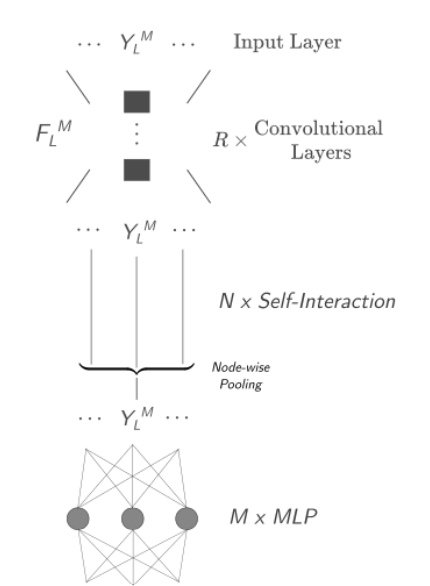
\includegraphics[scale=1.2]{model_arch.png}
%\end{center}
%\caption{Diagram depicting the general architecture of the model used in this work.  }
%\end{figure}


\subsection{Direct Prediction}
First, we consider a straight-forward prediction of the target tensor by training on the target set and then testing on some as-yet-unseen validation data. Results for these predictions are given in Figure \ref{direct}, with component-wise MAE presented in Figure \ref{heatmaps}.

While the average MAE for tensor components beats previous component-wise average results as reported in \cite{strainnet}, the heatmap displaying component-wise MAE suggest explicit incorporation of symmetry class information is necessary to further improve results.

\begin{figure}
\begin{center}
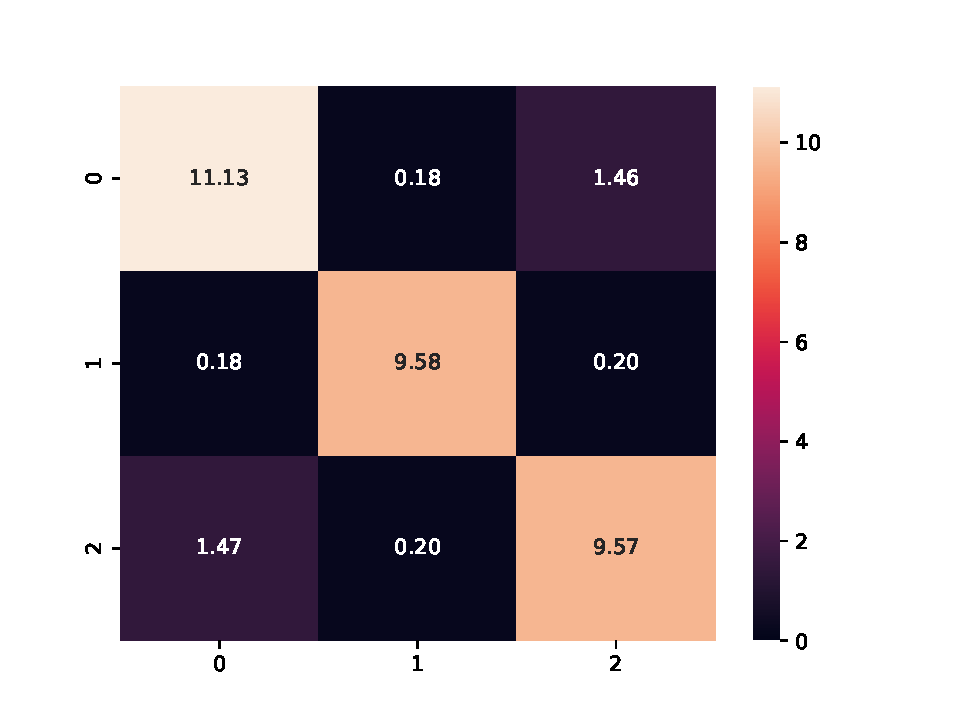
\includegraphics[scale=.3]{segnn_default_dielectric_heatmap.pdf}
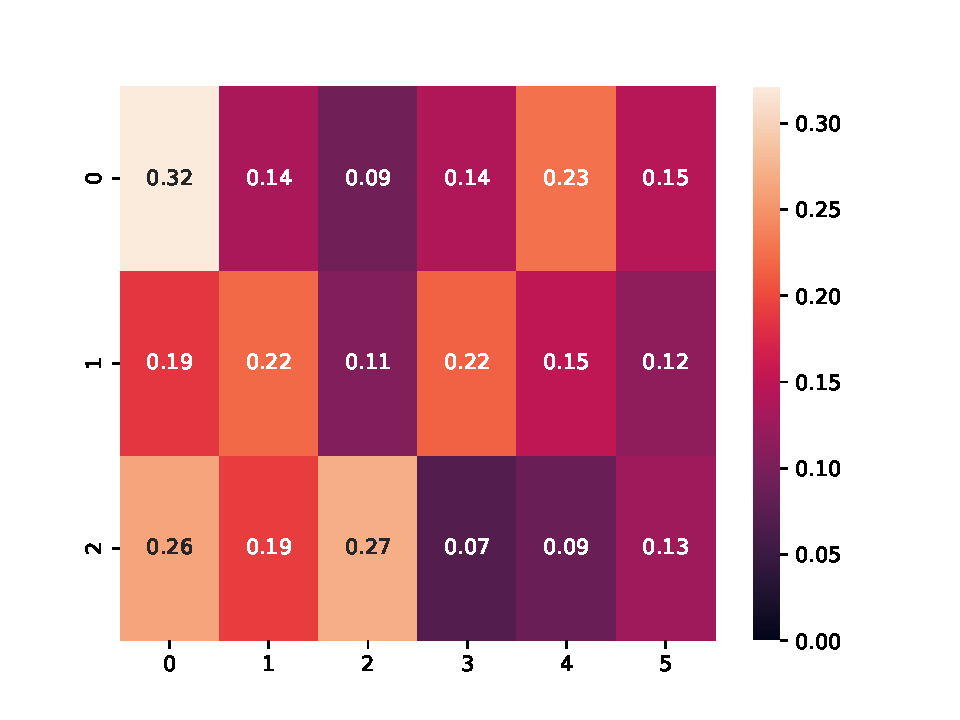
\includegraphics[scale=.3]{segnn_default_piezo_heatmap.pdf}
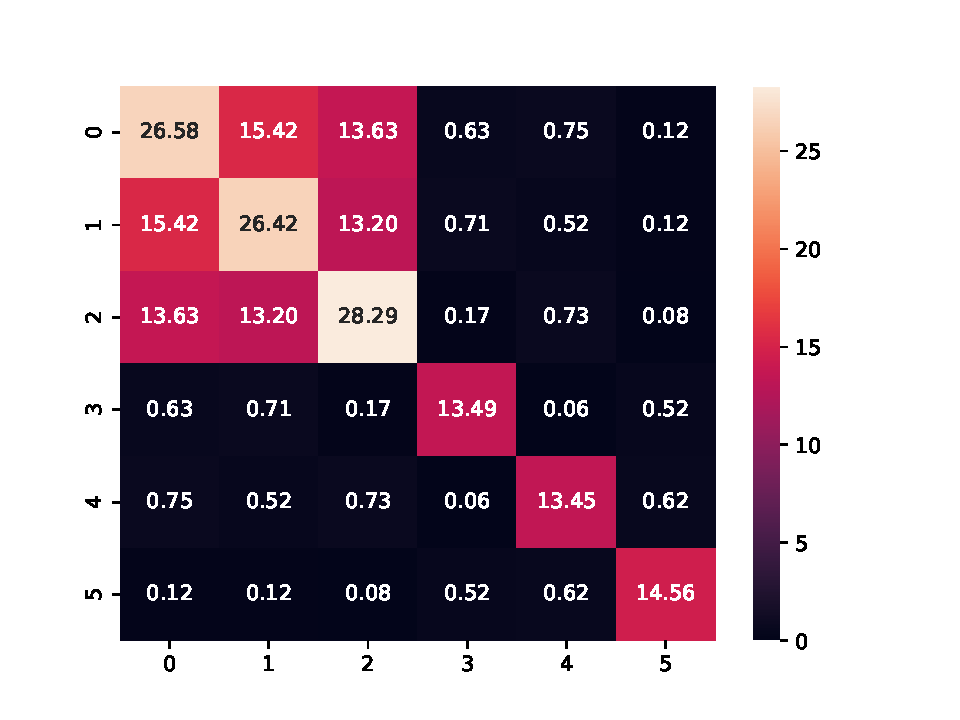
\includegraphics[scale=.3]{segnn_default_elastic_heatmap.pdf}
\end{center}
\caption{Heatmaps showing the component-wise MAE in Voigt notation for the all direct prediction tasks. Shown in order of dielectric, piezoelectric, and elastic tensor components. }\label{heatmaps}
\end{figure} 

\begin{figure}
\begin{tabular}{|c|ccc|}
\hline
& & MAE (Averaged Over Components)  & \\
Target Components & SEGNN & SEConv & SETransformer\\
\hline 
Elastic  \textit{[log$_10$(GPa)]}& 8.139 & 7.689 & 7.941 \\
Dielectric & 4.82 &4.702 &4.718\\
Piezoelectric \textit{[C/$m^2$]} & 0.170 & 0.170 & 0.1714\\
\hline
\end{tabular}
\caption{Results for direct prediction of elastic, piezoelectric, and dielectric tensor components. }\label{direct}
\end{figure}


\subsection{Transfer Learning Applications}
As a basic investigation into the broader usefulness of the trained models, we also test pretrained models on successive tasks and compare performance.

Pretraining may be particularly useful in the case of target sets with a limited number of data. As such, our experiments focus on a filter-down approach, in which we start training on larger datasets and then transfer the trained graph network weights to a downstream task with a smaller dataset (while continuing to train the transfered graph network).

Since all tensorial data is relatively restricted in terms of the total number of samples, the first transfer learning experiment consisted of pretraining a graph network on as large a dataset as possible, namely scalar data, and then transferring this model to different tensorial tasks. That is, we first consider a training progression:
$$
\textit{Scalar Target} \rightarrow \textit{Tensor Target},
$$
and compare results in Table \ref{fig:scalar2tensor}. The larger scalar datasets were the predicted formation energy per atom for a crystal, and the calculated band gap. Note that in these progressions, no data was witheld in the scalar target pretraining process.

In general though, pretraining of this nature had little effect on down-stream results. This may result from a number of factors. Perhaps there is too little overlap between the crystal structures of the smaller datasets and those of the larger dataset, so that the pretraining overgeneralizes the model to a larger class of materials than are relevant. The difference in rotational order between tasks may furthermore result in little overlap between the pre-trained filter weights and the down-stream task's pathway through the model. And, the relevance of certain tasks to one another may be hard to determine a priori.

\begin{figure}
\begin{tabular}{|c|c|ccc|}
\hline
&  & & MAE (Avg. over components) &\\
\textit{Pretraining Task:} & \textit{Tensor Target}  & SEGNN & SEConv & SETransformer\\
\hline
 & Elastic \textit{[log$_{10}$(GPa)]} & 8.19 \textit{(8.14)} &  7.98 \textit{(7.69)} & 7.65 \textit{(7.94)}\\
Formation Energy & Dielectric & 5.02 \textit{(4.82)} & 4.52 \textit{(4.71)} & 4.41 \textit{(4.72)} \\
& Piezoelectric \textit{[C$/m^2$]} & 0.170 \textit{(0.170)} & 0.170 \textit{(0.170)} & 0.171 \textit{(0.171)}\\
\hline
 & Elastic \textit{[log$_{10}$(GPa)]} & 8.39 \textit{(8.14)} &  7.87 \textit{(7.69)} & 8.34 \textit{(7.94)}\\
Band Gap & Dielectric & 4.74 \textit{(4.82)} & 4.35 \textit{(4.71)} & 4.56 \textit{(4.72)} \\
& Piezoelectric \textit{[C$/m^2$]} & 0.170 \textit{(0.170)} & 0.170 \textit{(0.170)} & 0.171 \textit{(0.171)}\\
\hline
\end{tabular}
\caption{Results for tensor component prediction accuracy  after pretraining on a scalar-target task for  materials. Numbers italicized in parentheses are the original accuracies (without pretraining).}\label{fig:scalar2tensor}
\end{figure}

The smallest dataset considered here is that of piezoelectric strain constants. Performance did not significantly improve with any scalar target pretraining in any of the models for this task. The scarcity of data for this target motivates a search for further improvement from larger, adjacent datasets.
The experiments performed to this end focused on three different training progressions of tasks:
\begin{itemize}
\item Band gap $\rightarrow$ Dielectric $\rightarrow$ Piezoelectric
\item Band gap $\rightarrow$ Elastic  $\rightarrow$ Piezoelectric
\item Band gap $\rightarrow$ Elastic $\rightarrow$ Dielectric $\rightarrow$ Piezoelectric
\end{itemize}
All failed to significantly improve performance in terms of MAE across tensor components.

\subsection*{Conclusion}

In a certain sense, the component-wise results and lack of transferability may indicate that the spherical harmonic approach is potentially 'too big' or too expressive to effectively predict crystalline material properties in a way that naturally respects crystalline symmetries. Indeed, $SO(3)$ convolution, as described here, generates a large set of unwanted and consequently discarded combinations of spherical harmonics. 

A simple approach would be to mask results according to crystal system, or build an individual model for each different crystal system with a unique output structure. However, a more unified approach might be to restrict convolution specifically to the crystal group elements. Future works may consider the symmetry of crystalline systems in such a way, so that we may avoid predicting tensor components that should be identically zero a priori. 


\nocite{*}
\bibliographystyle{annotate}
\bibliography{paper-spherical-elastic.bib}

\appendix



\section{Full Decompositions of Tensors}\label{decomps}
Below, we give the total decomposition of the three tensors of interest here. Namely, the rank-two dielectric tensor $\epsilon$, the rank-three piezoelecrtic strain tensor $d$, and the rank-four elastic tensor $C$. Each begins with the Young diagrams for the total rank tensor space and then uses the symmetries of the respective tensor to restrict down to the relevant Young tableux. These are used to form symmetrizers and then further decomposed with contractions with the metric tensor $g$ and the levi-civita tensor $\epsilon$ until all that remains are a set of fully symmetric sub-tensors.
\subsection{Dielectric Tensor Decomposition}
The decomposition of the dielectric tensor is essentially trivial since it is already symmetric. However, we give a detailed overview here for instructive purposes.

The GL decomposition of a rank-two tensor space is the usual symmetric-antisymmetric decomposition of a matrix $M$.
$$
M_{ij} = S_{ij} + A_{ij}\quad
$$
\begin{center}
with:
\begin{align*}
S_{ij}&=\frac{1}{2}(M_{ij}+M_{ji})\quad \Rightarrow\quad S_{ij}=S_{ji}\\
A_{ij}&=\frac{1}{2}(M_{ij}-M_{ji})\quad \Rightarrow\quad A_{ij}=-A_{ji}\\
\end{align*}
which correspond to the Young diagrams below:

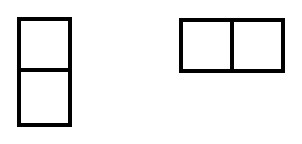
\includegraphics[scale=0.7]{rank2_young.pdf}.
\end{center}
Since the dielectric tensor $\epsilon$ is symmetric, we are left then only with the unique tableaux below, corresponding to the fully symmetric part $S$.
\begin{center}
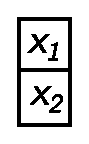
\includegraphics[scale=0.7]{dielectric_young.pdf}
\end{center}
We can then further decompose this rank-two symmetric into a rank-zero space and a rank-two space by taking the rank-0 trace $t = g_{ij}\epsilon_{ij}$ and then forming the rank-2 traceless residue $R_{ij}=\epsilon_{ij}-t\delta_{ij}$.
\subsection{Piezoelectric Tensor Decomposition}
The Young diagrams for a rank-three tensor are as follows:
\begin{center}
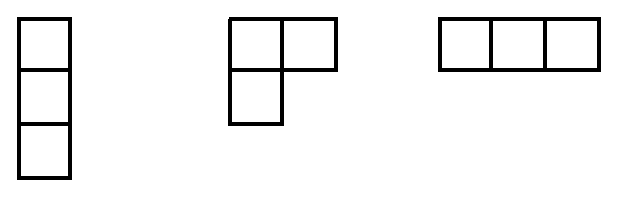
\includegraphics[scale=0.7]{youngdiagrams3.pdf}
\end{center}
according to the symmetry$d_{ijk}=d_{ikj}$, we can again see that all Young tableaux but the following will disappear, since the rest are asymmetric in the last two indices.
\begin{center}
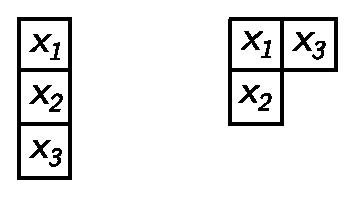
\includegraphics[scale=0.7]{piezo_young.pdf}
\end{center}
where the totally symmetric component tensor here we define as $S$ and the mixed symmetry component tensor we define $A$, so that we have the Young decomposition:
$$
d_{ijk} = S_{ijk}+A_{ijk}
$$
defined component-wise in terms of strain components:
\begin{align*}
S_{ijk}&=\frac{1}{3}\big(d_{ijk}+d_{ikj}+d_{kji}\big)\\
A_{ijk}&=\frac{1}{3}\big(2d_{ijk}-d_{ikj}-d_{kji}\big)\\
\end{align*}

The fully symmetric part $S$ is of an adequate form for harmonic decomposition, with those relations given in the next section.

The mixed symmetry part $A$ however requires further decomposition with respect to $SO(3)$, so that we have a set of symmetric tensors describing it. It's 8 independent components can be described by a $5\oplus 3$ dimensional space consisting of a symmetric rank-2 tensor and a trace vector.

The trace vector $v^i$, describing $A$'s 3-dimensional $SO(3)$ invariant subspace, can be formed from the contraction of the metric tensor $g$ along $A$'s first and second indices. That is, we define:
$$
v^i =g_{jk}A^{ijk}
$$
Note that this choice is somewhat arbitrary, since we could define the trace part to correspond to the contraction along the first and third indices, or the second and third. However, it can be shown that for the mixed symmetry of $A$, these two potential trace vectors are linearly dependent (related by an overall factor of $1$ and $-2$, respectively).

Rather simply then, we can reconstruct a third-rank tensor $V$, corresponding to this rank-one invariant subspace, by defining $V$ component-wise as:
$$
V_{ijk} =\frac{1}{4}\big[v_i g_{jk}+ v_j g_{ik} - 2 v_j g_{ik}\big]
$$
The rank-2 invariant subspace of $A$ then may be constructed by symmetrizing the partial contraction with $\epsilon$ along the first and second indices (the anti-symmetric pair). Note that the antisymmetric part of this partial contraction corresponds to the trace vector space accounted for here by $u$. Explicitly, we define:
$$
b_{ij}=\frac{1}{2}\big(\epsilon_{i}^{mk}A_{mkj}+\epsilon_{j}^{mk}A_{mki}\big)
$$
which is a traceless symmetric rank-2 tensor. And from which we may reconstruct the corresponding rank-3 tensor $B$, defined by:
$$
B_{ijk}=\frac{1}{3}\big[ \epsilon_{ik}^p b_{pj}+\epsilon_{ij}^p b_{pk}\big]
$$
Thus, we may provide a total harmonic decomposition for $A$ in terms of the invariant subspaces of the rank-1 $u$ and the rank-2 $b$, such that:
$$
A_{ijk} = V_{ijk} + B_{ijk}
$$
And so, as mentioned above, the symmetric part $S$ is readily decomposed in the spherical bases into $\mathcal{H}^{(1)}\oplus \mathcal{H}^{(3)}$. And then the mixed-symmetry part inhabits the space $\mathcal{H}^{(1)}\oplus \mathcal{H}^{(2)}$.


\subsection{Elastic Tensor Decomposition}

If we examine the Young diagrams of a fourth rank tensor, as below: 

\begin{center}
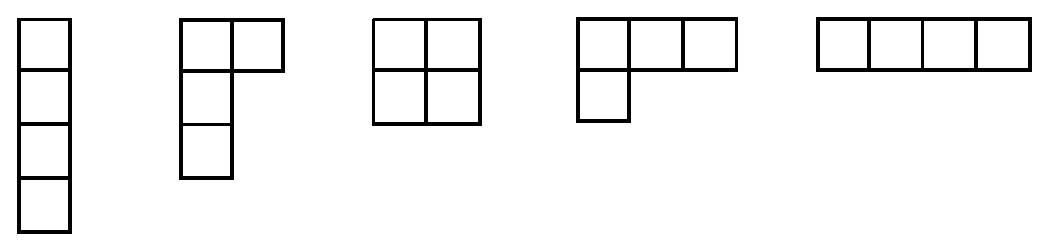
\includegraphics[scale=0.7]{rank4_young.pdf}
\end{center}
We can immediately notice that the symmetries of $C$ require that all but the totally symmetric tensor $S$ and one mixed symmetry tensor $A$ must vanish. $S$ has 15 independent components, and $A$ has 6. Furthermore, $A$ has corresponding symmetrizer $\mathcal{C}S(x_1x_2)S(x_3x_4)A(x_1x_3)A(x_2x_4)$. Thus, $A$ is exactly the tensor symmetric under permutation of $i,j$ and $k,l$ but antisymmetric under exchanges $i,k$ and $j,l$.
\begin{center}
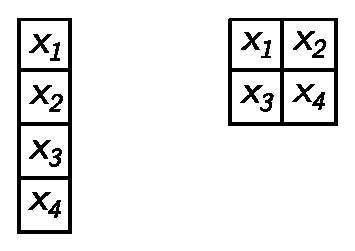
\includegraphics[scale=0.7]{elastic_young.pdf}
\end{center}
Note that this mixed-symmetry subspace $A$ corresponds to Backus' \cite{backus1970geometrical} asymmetric tensor $A$. With $S$ and $A$ being defined component-wise as:
$$
S_{ijkl}=\frac{1}{3}\big( C_{ijkl} + C_{ikjl} + C_{klij} \big)
$$
$$
A_{ijkl} = \frac{1}{3}\big( 2C_{ijkl} -C_{ikjl} -C_{klij}  \big)
$$
The fully symmetric part can of course be converted to spherical harmonic components via a Clebsch-Gordon expansion. The mixed symmetry $A$, however requires further decomposition. 

All six components can be described by the symmetric (but not traceless) tensor $t$, defined as the double partial contraction of $A$ with the totally antisymmetric tensor $\epsilon$ as:
$$
t_{ij} = \epsilon_{i}^{mk}\epsilon_{j}^{nl}A_{mnkl}
$$
\begin{center}
which can be reconstructed as the subtensor $N$ as:
\end{center}
$$
N_{ijkl}= \frac{1}{2}\big(\epsilon^{}\epsilon^{} - \epsilon^{} \epsilon^{} \big)t_{mn}
$$
This tensor $t$ then has a harmonic decomposition according to the rank-two Clebsch-Gordon transformation between the $J_z$ basis and the harmonic basis $y_{\ell}^m$. 




\begin{figure}
\section{Table of Coefficients for $J_z\rightarrow y_{\ell}^m$ Transformation}\label{cgcoef}
\begin{tabular}{c|ccccccc}
$\mathbf{Rank\ 2}$ \\
\hline
& $a_{00}$ & $a_{+-}$ & $a_{0\pm}$ & $a_{\pm\pm}$ \\
$y_0^0$  & $1$ & $-2$ \\
$y_2^0$  & $1$ & $1$ \\
$y_2^{\pm 1}$  &  & & $\sqrt{3}$ \\
$y_2^{\pm 2}$  &  & & & $\sqrt{\frac{3}{2}}$
\\
\\
\\
$\mathbf{Rank\ 3}$\\
\hline
 & $a_{000}$ & $a_{0+-}$ & $a_{00\pm}$ & $a_{+-\pm}$  & $a_{0\pm\pm}$ & $a_{\pm\pm\pm}$ \\
$y_1^0$  & $3$ & $-6$ \\
$y_3^0$  & $\frac{15}{7}$ & $-\frac{5}{7}$ \\
$y_1^{\pm 1}$  &  & & $\sqrt{\frac{3}{2}}$ & $-2\sqrt{\frac{3}{2}}$\\
$y_3^{\pm 1}$  &  & & $2\sqrt{\frac{3}{2}}$ & $\sqrt{\frac{3}{2}}$\\
$y_3^{\pm 2}$  &  & & & & $\sqrt{\frac{15}{2}}$\\
$y_3^{\pm 3}$  &  & & & & & $\sqrt{\frac{5}{2}}$\\
\\
\\
\\
\textbf{Elastic}\\
(Rank 4) \\
 \hline 
$(m=0)$& $a_{0000}$ & $a_{00+-}$ & $a_{0+0-}$ & $a_{+-+-}$  & $a_{++--}$ \\
$y_0^{0}$  & $1$ & $2$ &$-6$ & 1 & 3 \\
$y_2^0$  & 1 & $2$ & $-3$ & 1 & $-3$\\
$y_4^0$ & 1 & $2$ & $4$ & 1 & $\frac{1}{2}$\\
 \\
$(m=1,2)$& $a_{000\pm}$ & $a_{+- 0 \pm}$  & $a_{\mp 0 \pm\pm}$ & $a_{00\pm\pm}$ & $a_{+- \pm \pm}$  & $a_{\mp \pm \mp\pm}$ \\
$y_2^{\pm 1}$  & $\sqrt{3}$ & $\sqrt{3}$ &  $-3\sqrt{3}$\\
$y_4^{\pm 1}$  & $2\sqrt{\frac{5}{2}}$ & $2\sqrt{\frac{5}{2}}$ & $\sqrt{\frac{5}{2}}$  \\
$y_2^{\pm 2}$  & & & & $-2\sqrt{\frac{3}{2}}$ & $-2\sqrt{\frac{3}{2}}$ & $3\sqrt{\frac{3}{2}}$  \\
$y_4^{\pm 2}$ & & & & $\sqrt{\frac{5}{2}}$ & $\sqrt{\frac{5}{2}}$ & $2\sqrt{\frac{5}{2}}$  \\
\\
$(m=3,4)$& $a_{\pm\pm\pm 0}$ & $a_{\pm\pm\pm\pm}$  \\
$y_4^{\pm 3}$  & $\sqrt{\frac{35}{2}}$ &  \\
$y_4^{\pm 4}$  &  & $\frac{1}{2}\sqrt{\frac{35}{2}}$\\ 
\end{tabular}
\caption{Coefficients for transformation between spherical basis components $a_{\alpha\beta\gamma\delta}$ and harmonic components $y^m_l$ for a rank-2,3,4 symmetric tensor. Note that the rank-4 is only relevant for symmetric components of elastic tensors and correspond to Mochizuki's transformation \cite{mochizuki1988spherical} between the $J_z$ basis and their symmetric tensor $s$.}
\end{figure}

\section{Real Spherical Harmonics}\label{realsph}
The (complex) spherical harmonics $Y_{\ell}^m$ can be transformed into a set of real spherical harmonics $Y_{\ell m}$ according the following relations:
$$
Y_{\ell m }=
\begin{cases}
\frac{i}{\sqrt{2}}\big(Y_{\ell}^{-|m|} - (-1)^m Y_{\ell}^{|m|} \big):\ \ m<0\\
\quad\quad\quad\quad Y_{\ell}^0:\quad\quad\quad\quad\quad\ \ \  \ m=0\\
\frac{1}{\sqrt{2}}\big(Y_{\ell}^{-|m|} + (-1)^m Y_{\ell}^{|m|} \big):\ \ m>0\\
\end{cases}
$$
(of course, this choice is not entirely unique, with the choice made here assuming a Condon-Shortley phase included in the definition of $Y_{\ell}^m$).



\end{document}